\subsection{M.PC.MS - Metriche Soddisfatte}
\label{sec:MS}

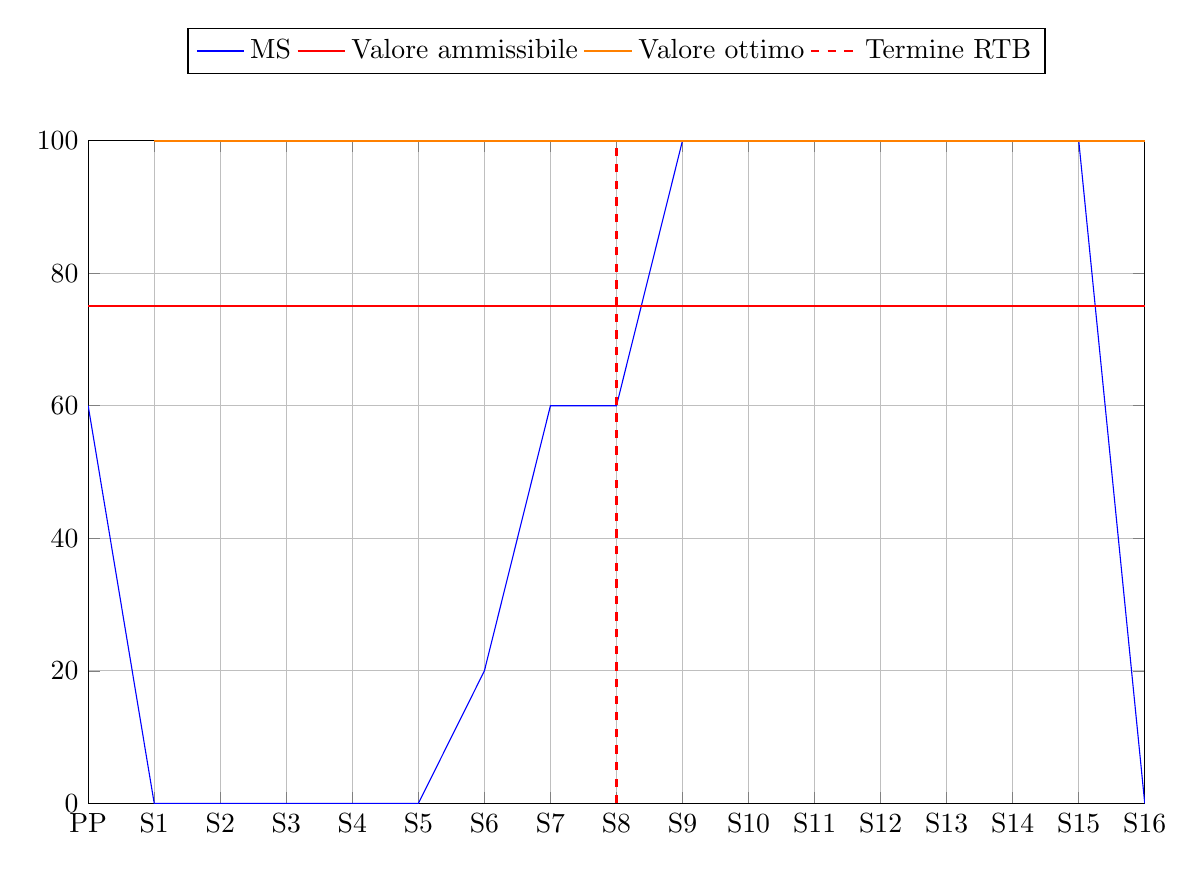
\begin{tikzpicture}
    \begin{axis}[
        width=15cm, height=10cm,
        ymin=0, ymax=100,
        xmin=0, xmax=16,
        xtick={0, 1, 2, 3, 4, 5, 6, 7, 8, 9, 10, 11, 12, 13, 14, 15, 16},
        xticklabels={PP, S1, S2, S3, S4, S5, S6, S7, S8, S9, S10, S11, S12, S13, S14, S15, S16},
        xlabel={},
        ylabel={},
        grid=major,
        scaled ticks=false,
        legend style={at={(0.5,1.1)}, anchor=south, legend columns=-1},
    ]
    \addplot[color=blue] coordinates {(0, 60) (1, 0) (2, 0) (3, 0) (4, 0) (5, 0) (6, 20) (7, 60) (8, 60) (9, 100) (10, 100) (11, 100) (12, 100) (13, 100) (14, 100) (15, 100) (16, 0)};
    \addlegendentry{MS}
    \addplot[red, thick] coordinates {(0, 75) (17, 75)};
    \addlegendentry{Valore ammissibile}
    \addplot[orange, thick] coordinates {(1, 100) (17, 100)};
    \addlegendentry{Valore ottimo}
    \addplot[red, thick, dashed] coordinates {(8, 0) (8, 100)};
    \addlegendentry{Termine RTB}
    \end{axis}
\end{tikzpicture}
\subsubsection{RTB}
Non è stata assicurata la qualità che si voleva raggiungere per la realizzazione del progetto, i valori inferiori al valore ammissibile sono dovuti
dalle \glossario{metriche} di \glossario{Schedule Variance}, \glossario{Cost Variance}, Correttezza ortografica e Variazione del Piano che non hanno mai raggiunto il valore ammissibile durante lo svolgimento del progetto 
indicando una metodologia di lavoro che non è migliorata sufficientemente con il passare del tempo.

\paragraph{Sprint 9}
Durante lo \glossario{Sprint} 9 sono state soddisfatte tutte le metriche attualmente previste per il progetto, grazie a un miglioramento della pianificazione e dell'assegnazione delle attività. 

\paragraph{Sprint 10}
Durante lo \glossario{Sprint} 10 sono state soddisfatte tutte le metriche attualmente previste per il progetto. 

\paragraph{Sprint 11}
Durante lo \glossario{Sprint} 11 sono state soddisfatte tutte le metriche attualmente previste per il progetto. 

\paragraph{Sprint 12}
Durante lo \glossario{Sprint} 12 sono state soddisfatte tutte le metriche attualmente previste per il progetto. 

\paragraph{Sprint 13}
Durante lo \glossario{Sprint} 13 sono state soddisfatte tutte le metriche attualmente previste per il progetto.

\paragraph{Sprint 14}
Durante lo \glossario{Sprint} 14 sono state soddisfatte tutte le metriche attualmente previste per il progetto.

\paragraph{Sprint 15}
Durante lo \glossario{Sprint} 15 sono state soddisfatte tutte le metriche attualmente previste per il progetto.

\paragraph{Sprint 16}
Sebbene i valori delle metriche siano stati soddisfatti, il progetto non è stato completato entro il termine delle risorse disponibili,
portando a un valore di MS pari a 0. Questo indica che, nonostante il lavoro svolto, il progetto non ha raggiunto gli obiettivi prefissati entro il termine stabilito.